\documentclass{amsart}

%%%%%%%%%%%%%%%%%%%%%%%%%%%%%%%%%%%%%%

\usepackage[utf8]{inputenc}
\usepackage[T1]{fontenc}

\usepackage{a4wide}%en grand
\usepackage{changepage}%indentation

\usepackage{xcolor}
\usepackage{amsfonts,amsthm,amssymb,amsmath}
\usepackage{mathtools}
\usepackage{wasysym}
\usepackage{xspace}
\usepackage{graphicx}
%\usepackage[notcite,notref]{showkeys} % shows labels 
\usepackage{breqn}
\usepackage{algorithm}
\usepackage{algorithmic}
\usepackage{tabularx}

\usepackage[english]{babel} %gestion des langues
\usepackage{caption}
\usepackage{subcaption}
\usepackage{paralist}
\usepackage{multirow}

\usepackage{hyperref}
\hypersetup{colorlinks=true, citecolor=darkblue, linkcolor=darkblue}
\usepackage{hypcap}

\usepackage[noabbrev,capitalise]{cleveref}
\usepackage{autonum}
\usepackage{xspace}

%%%%%%%%%%%%%%%%%%%%%%%%%%%%%%%%%%%%%%

\newtheorem{theorem}{Theorem}[section]
\newtheorem{proposition}[theorem]{Proposition}
\newtheorem{lemma}[theorem]{Lemma}
\newtheorem{ce}[theorem]{Counter-example}
\newtheorem{claim}[theorem]{Claim}
\newtheorem{corollary}[theorem]{Corollary}
\newtheorem{definition}[theorem]{Definition}
\newtheorem{notation}[theorem]{Notation}
\theoremstyle{remark}
\newtheorem{remark}{Remark}[section]
\newtheorem{example}{Example}
\newtheorem{algo}{Algorithm}
\newtheorem*{example*}{Example}

\crefname{theorem}{Theorem}{Theorems}
\crefname{lemma}{Lemma}{Lemmas}

\definecolor{darkblue}{rgb}{0,0,0.7} % darkblue color
\newcommand{\darkblue}{\color{darkblue}} % darkblue command
\newcommand{\defn}[1]{\textsl{\darkblue #1}} % emphasis of a definition

%%%%%%%%%%%%%%%%%%%%%%%%%%%%%%%%%%%%%%

\newcommand*{\dual}[1]{{#1^*}}
\newcommand*{\nbd}[0]{neighbourhood\xspace}
\newcommand*{\ef}[0]{E-finite\xspace}
\newcommand*{\vf}[0]{V-finite\xspace}
\newcommand*{\ktg}[0]{$k$-triangulation\xspace}

\newcommand{\cl}{\prec}
\newcommand{\cle}{\preccurlyeq}

\newcommand{\surface}{\mathcal{S}}

\newcommand{\set}[2]{\left\{ #1 \;\middle|\; #2 \right\}} % set notation
\newcommand{\bigset}[2]{\big\{ #1 \;\big|\; #2 \big\}} % big set notation
\newcommand{\Bigset}[2]{\Big\{ #1 \;\Big|\; #2 \Big\}} % Big set notation
\newcommand{\setangle}[2]{\left\langle #1 \;\middle|\; #2 \right\rangle} % set notation
\newcommand{\ssm}{\smallsetminus} % small set minus
\newcommand{\dotprod}[2]{\left\langle \, #1 \; \middle| \; #2 \, \right\rangle} % dot product
\newcommand{\symdif}{\,\triangle\,} % symmetric difference
\newcommand{\one}{{1\!\!1}} % the all one vector
\newcommand{\eqdef}{\mbox{\,\raisebox{0.2ex}{\scriptsize\ensuremath{\mathrm:}}\ensuremath{=}\,}} % :=
\newcommand{\defeq}{\mbox{~\ensuremath{=}\raisebox{0.2ex}{\scriptsize\ensuremath{\mathrm:}} }} % =:
\newcommand{\viceversa}{\textit{vice versa}} % vice versa

\graphicspath{{../figures/}}
\graphicspath{{figures/}}

% marginal comments
\usepackage{todonotes}
\newcommand{\vincent}[1]{\todo[color=blue!30]{#1 \\ \hfill --- V.}}
\newcommand{\mathias}[1]{\todo[color=red!30]{#1 \\ \hfill --- M.}}

%%%%%%%%%%%%%%%%%%%%%%%%%%%%%%%%%%%%%%

\title[Infinite multitriangulations and multitriangulations of surfaces]{Infinite multitriangulations \\ and multitriangulations of surfaces}

\thanks{ML was partially supported by the French ANR grant GATO~(16\,CE40\,0009). \\ \indent VP was partially supported by the French ANR grants SC3A~(15\,CE40\,0004\,01) and CAPPS~(17\,CE40\,0018).}

\author{Mathias Lepoutre}
\address{LIX, \'Ecole Polytechnique, Palaiseau}
\email{mathias.lepoutre@lix.polytechnique.fr}
\urladdr{\url{http://www.lix.polytechnique.fr/Labo/Mathias.Lepoutre/}}

\author{Vincent Pilaud}
\address{CNRS \& LIX, \'Ecole Polytechnique, Palaiseau}
\email{vincent.pilaud@lix.polytechnique.fr}
\urladdr{\url{http://www.lix.polytechnique.fr/~pilaud/}}

%%%%%%%%%%%%%%%%%%%%%%%%%%%%%%%%%%%%%%

\begin{document}

\begin{abstract}
We extend previous work on the structure of $k$-stars of a multi-triangulation on a convex polygon to the case of multi-triangulations on any surface, orientable or not. 

To that extent, we use the universal cover construction, that makes a map on a surface into a periodic map of an infinite polygon. We generalize the work of Pilaud and Santos to multi-triangulation of an infinite polygon, with some additional constraints, and then conclude about the case of multi-triangulations on any surface.
\end{abstract}

\maketitle

\begin{figure}[h]
	\capstart
	\centerline{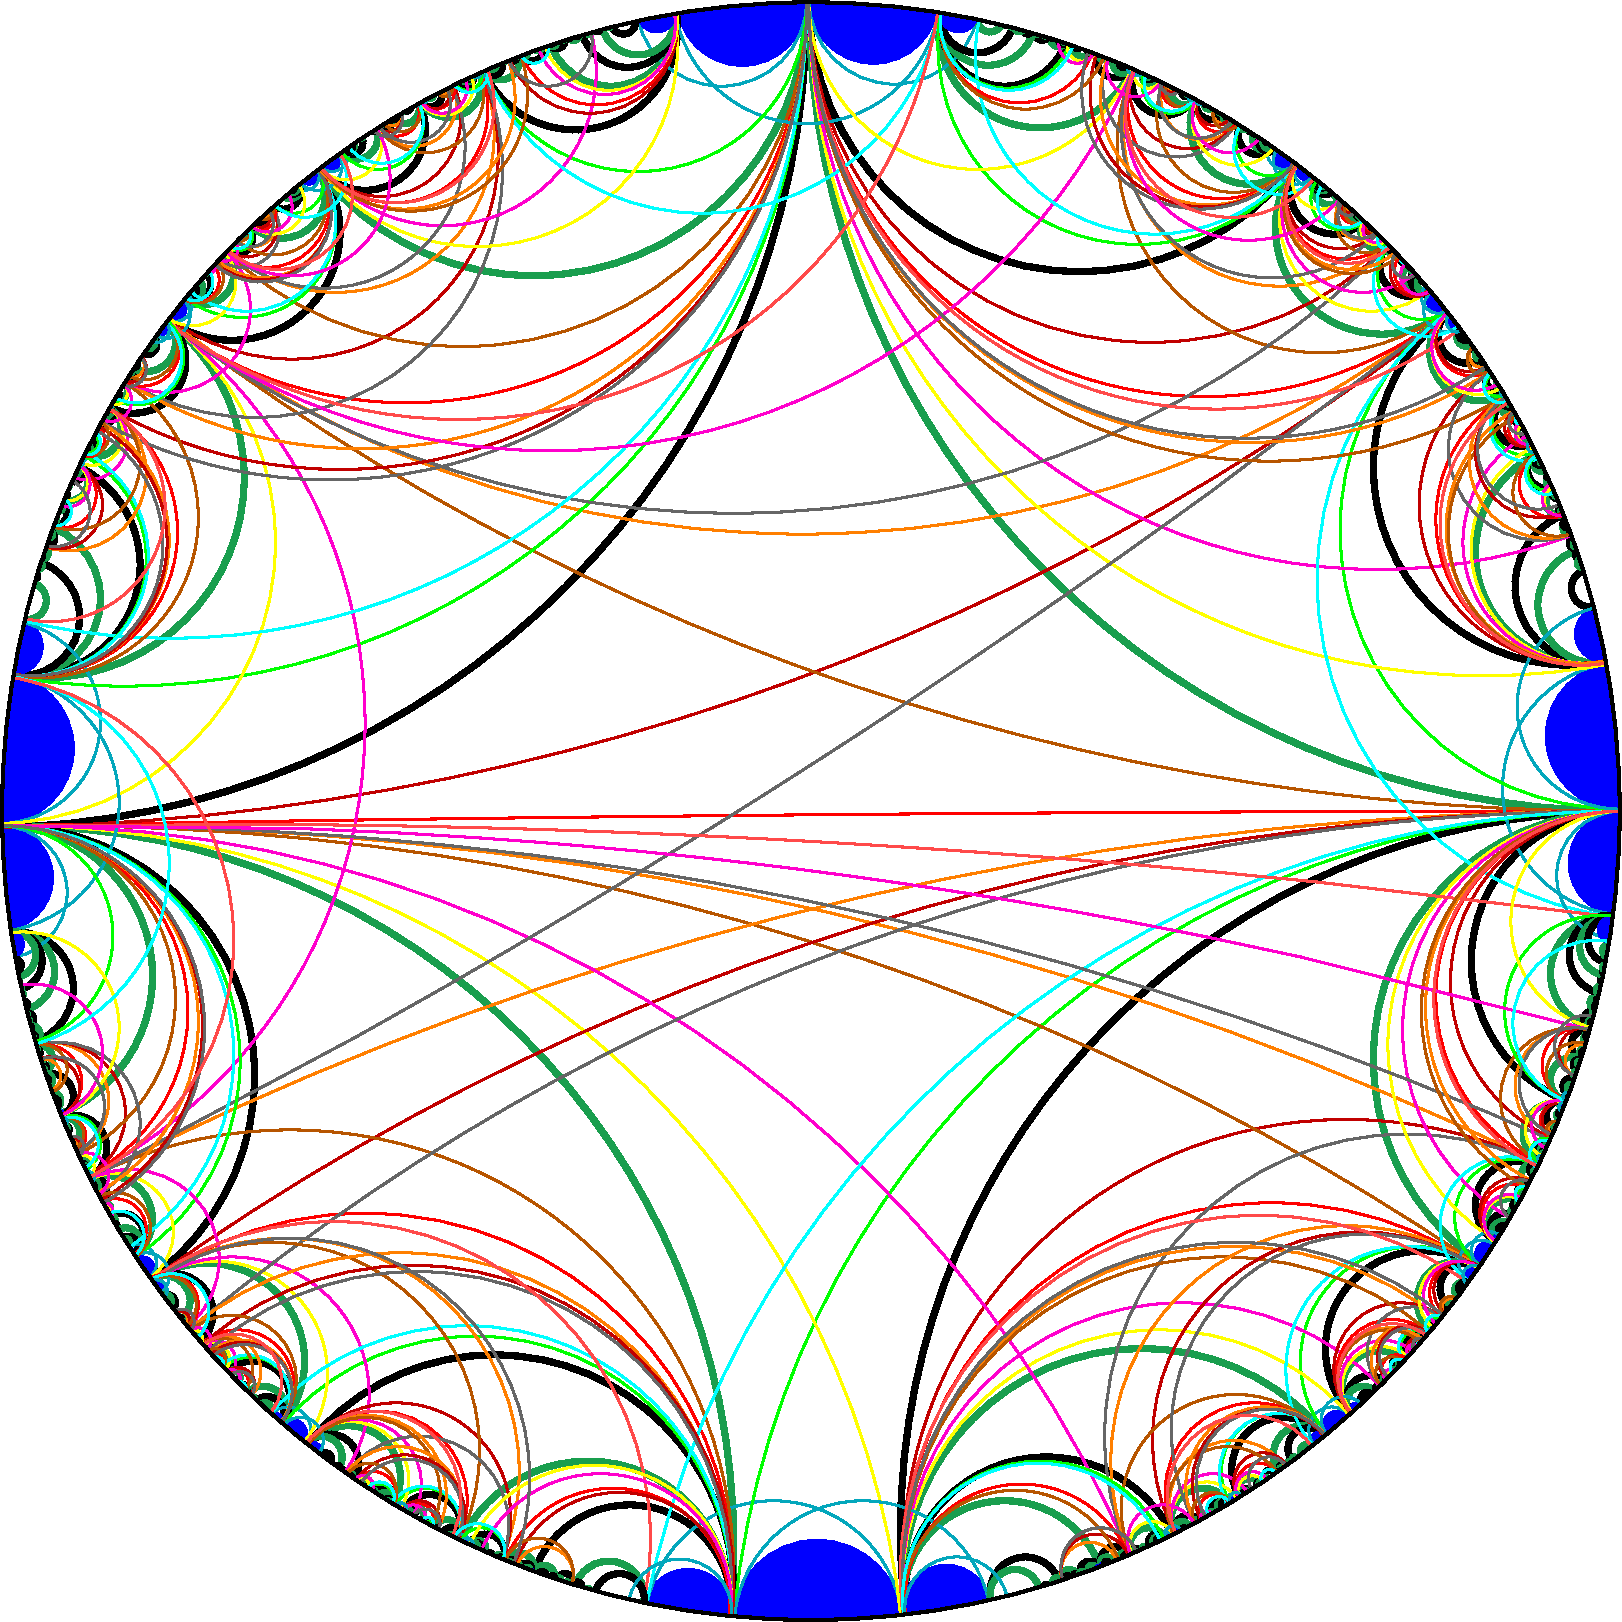
\includegraphics[scale=.42]{torusClean}}
	\caption{The universal cover of the $2$-triangulation of a torus with a hole, represented in \cref{fig:torus}}
	\label{fig:UCtorus}
\end{figure}


\section{Multitriangulations of infinite polygons}

\subsection{Infinite polygons}

\begin{definition}
A \defn{polygon}~$P$ is a cyclically ordered set, that might be finite or infinite.
We write~$a \cl b \cl c$ for the cyclic order.
The elements of~$P$ are called \defn{points} and pairs of elements of~$P$ are called \defn{diagonals}.
For two points~$a,b \in P$, let~$[a,b] \eqdef \set{c \in P}{a \le c \le b}$, and define similarly the intervals~$[a,b[$, $]a,b]$ and~$]a,b[$ (with open brackets for strict inequalitites).
Two diagonals~$(a,c)$ and~$(b,d)$ of~$P$ \defn{cross} if~$a \cl b \cl c \cl d$.
\end{definition}

\begin{definition}
If $x$ and $y$ are two points of a polygon~$P$ such that the interval~$]x,y[$ is empty, we say that~$x$ is the \defn{predecessor} of~$y$ and that~$y$ is the \defn{successor} of~$x$. A polygon~$P$ is \defn{tidy} if each point of~$P$ has both a predecessor and a successor. In particular, finite polygons are tidy.
\end{definition}

\begin{definition}
A set~$X$ of diagonals of a polygon~$P$ is 
\begin{itemize}
\item \defn{\ef} if each diagonal of~$X$ is crossed by a finite number of diagonals of~$X$,
\item \defn{\vf} if each vertex of~$P$ is incident to finitely many diagonals of~$X$.
\end{itemize}
\end{definition}

\begin{definition}[periodic]

\end{definition}

\subsection{Infinite multitriangulations}

\begin{definition}
A \defn{$k$-crossing} of a polygon~$P$ is a set of~$k$ pairwise crossing diagonals of~$P$.
A \defn{$k$-triangulation} of~$P$ is an inclusion maximal set of diagonals of~$P$ with no $(k+1)$-crossing.
\end{definition}

\begin{definition}
The \defn{length} of a diagonal~$(a,b)$ of a polygon~$P$ is the minimum~$\ell(a,b)$ of~$|{]a,b[}|$ and~$|{]b,a[}|$ (note that this might be infinite).
A diagonal~$(a,b)$ with~$\ell(a,b) > k$ (resp.~$\ell(a,b) = k$, resp.~$\ell(a,b) < k$) is a \defn{$k$-relevant} (resp.~\defn{$k$-boundary}, resp.~\defn{$k$-irrelevant}) diagonal.
\end{definition}

\begin{remark}
Observe that a diagonal contained in a $(k+1)$-crossing must be $k$-relevant.
Therefore, any \ktg contains all $k$-irrelevant and $k$-boundary diagonals by maximality.
\end{remark}


\begin{definition}
A \defn{$k$-star} of a polygon~$P$ is a set of diagonals of~$P$ of the form~$\set{(s_i, s_{i+k})}{0 \le i \le 2k}$ where~$s_0 \cl \dots \cl s_{2k}$ (the indices are understood modulo~$2k+1$).
\end{definition}

\begin{definition}
An \defn{angle} of a set~$X$ of diagonals of a polygon~$P$ is a pair of diagonals~$\{(u,v), (v,w)\}$ with~$u \cl v \cl w$ such that~$X$ contains no diagonal of the form~$(v,t)$ with~$w \cl t \cl u$. The angle is denoted by~$\angle(u,v,w)$ and we say that~$v$ is the \defn{apex} of~$\angle(u,v,w)$. An angle is \defn{$k$-relevant} if none of its diagonals is $k$-irrelevant. %A set~$Y$ of diagonals of~$P$ crosses the angle~$\angle(u,v,w)$ if each diagonal of~$Y$ crosses both~$(u,v)$ and~$(v,w)$. 
\end{definition}

One of the objectives of this paper is to prove the following structural results on infinite multitriangulations

\begin{theorem}
\label{thm:structureInfinite}
Let~$T$ be a \ef \ktg of a tidy polygon~$P$.
\begin{enumerate}
\item Each $k$-relevant angle of~$T$ is contained in precisely one $k$-star of~$T$.
\item Each $k$-relevant (resp.~$k$-boundary, resp.~$k$-irrelevant) diagonal of~$P$ is contained in precisely two (resp.~one, resp.~none) $k$-stars of~$T$.
\item For any $k$-relevant diagonal~$e$ of~$T$, there exists a unique diagonal~$f$ not in~$T$ such that~$T \symdif \{e,f\}$ is another $k$-triangulation. The diagonal~$f$ only depend on the two $k$-stars of~$T$ containing~$e$.
\item Let~$P'$ denote a polygon obtained by replacing $k+1$ consecutive points of~$P$ by~$k$ points. Then there exists a flattening (resp.~inflating) operation that transforms the \ktg{}s of~$P$ into the \ktg{}s of~$P'$ (resp.~and \viceversa).
\item For any point~$p$ of the plane, the $k$-depth of~$p$ in~$P$ is equal to the sum of the winding numbers around~$p$ of the $k$-stars of~$T$.
\vincent{Vrai ?}
\end{enumerate}
\end{theorem}

\begin{remark}
\begin{itemize}
\item flip graph connected? Increasing flip graph?
\item duality with pseudoline arrangements?
\item $k$-arboresence? connection to $k$-edge-connected but not locally $(k+1)$-edge-connected.
\end{itemize}
\end{remark}

\section{Multitriangulations of surfaces}

\begin{definition}
Consider an connected surface~$\surface$ with boundary and a set~$V$ of marked points on the boundary, with at least one marked point on each boundary component. An \defn{arc} of~$\surface$ is a curve on~$\surface$ connecting two points of~$V$ and whose interior is disjoint from the boundary of~$\surface$. We consider arcs up to homotopy relative to their endpoints in~$\surface$ and we disallow arcs homotopic to a boundary segment of~$\surface$.
\end{definition}

\begin{definition}
Universal cover~$\pi : \bar\surface \to \surface$.
\vincent{Not clear}
\end{definition}

\begin{definition}
A \defn{$k$-crossing} on~$\surface$ is a collection~$\alpha_1, \dots, \alpha_k$ of $k$ arcs of~$\surface$ which admit pairwise crossing representatives~$\bar\alpha_1, \dots, \bar\alpha_k$ in the universal cover~$\bar\surface$.
A \defn{$k$-triangulation} of~$P$ is an inclusion maximal set of diagonals of~$P$ with no $(k+1)$-crossing.
\end{definition}

\begin{remark}
Be careful: a $k$-crossing on~$\surface$ is NOT a collection of pairwise crossing arcs of~$\surface$. Namely, there are collections of pairwise crossing arcs of~$\surface$ which do not admit pairwise crossing representatives. The simplest examples are self-crossing arcs, since their representative are not self-crossing. Further examples are given in \cref{fig:notkcrossing}.
\vincent{Todo.}
\end{remark}

\begin{theorem}
\label{thm:structureSurface}
Any \ktg of a surface of genus~$g$ with~$b$ boundaries and~$n$ marked points has precisely $n + 2k(2g + b - 2)$ $k$-stars and $kn + k(2k + 1)(2g + b - 2)$ $k$-relevant arcs.
\end{theorem}


\begin{remark}
\begin{itemize}
\item \cite[Lem.~7.10]{PilaudSantos}: Any $k$-triangulation of the $n$-gon contains at most $k(n-2p-1)$ $p$-relevant diagonals. Extension for surfaces.
\item flip graph connected? Increasing flip graph? Is it a lattice? (use bracket vectors)
\item duality? Line space of the surface?
\item punctures?
\end{itemize}
\end{remark}


\begin{figure}[h]
	\capstart
	\centerline{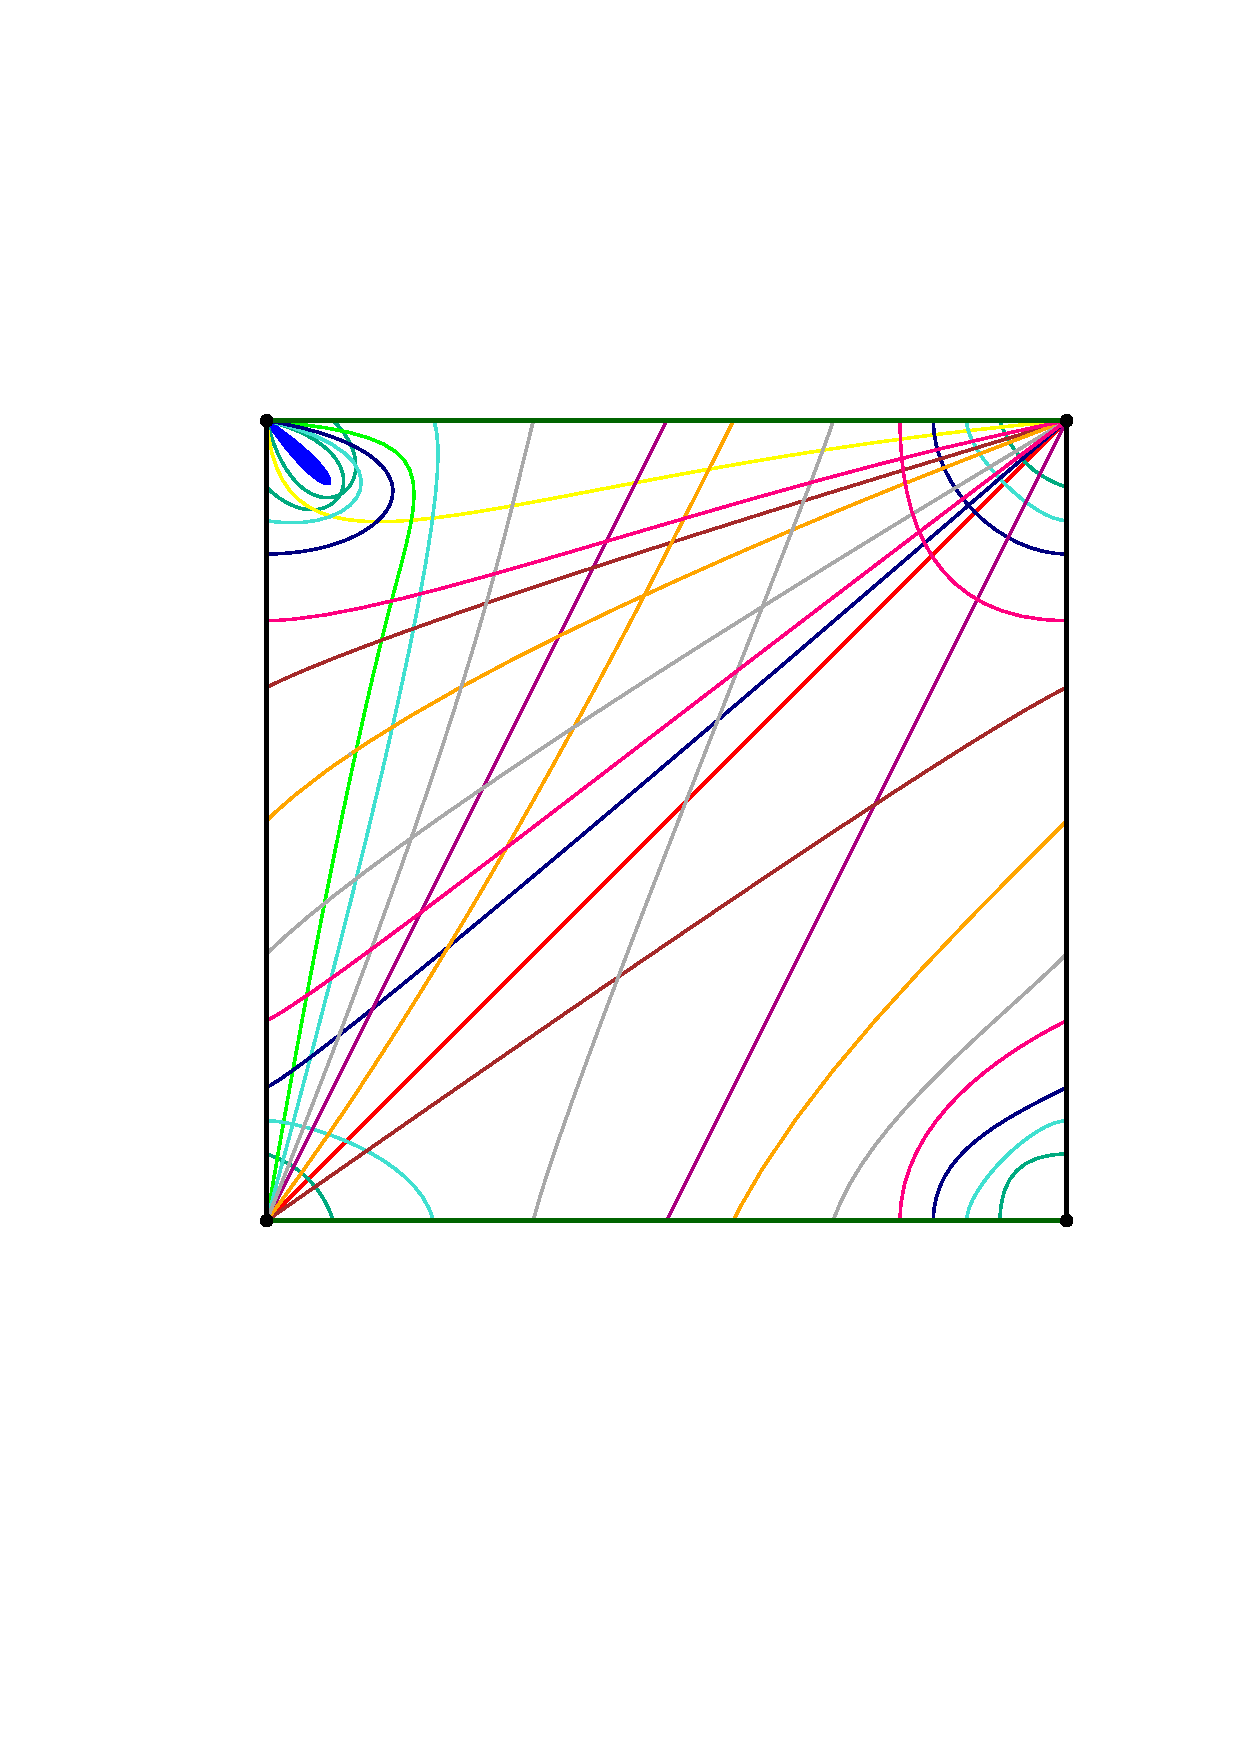
\includegraphics[scale=.42]{exTorusSquare}}
	\caption{A $2$-triangulation of a torus with a hole (in blue), whose universal cover is represented in \cref{fig:UCtorus}}
	\label{fig:torus}
\end{figure}

\subsection{Cylinder with two points on one boundary and none on the other}



\section{Proof of \cref{thm:structureInfinite}}

\subsection{$(k-1)$-crossings crossing an angle}

We say that a $(k-1)$-crossing~$A = \{a_1, \dots, a_{k-1}\}$ crosses an angle~$\angle(u,v,w)$ if each diagonal~$a_i$ crosses both~$(u,v)$ and~$(v,w)$. We stick to the convention to label the diagonals of~$A$ in such a way that $u \cl a^\bullet_1 \cl \dots \cl a^\bullet_{k-1} \cl v \cl a^\circ_1 \cl \dots \cl a^\circ_{k-1} \cl w$. We use this convention throughout this section without further notice.

\begin{lemma}
\label{lem:tidyExists}
In a \ktg of a tidy polygon, any $k$-relevant angle is crossed by a $(k-1)$-crossing.
\end{lemma}

\begin{proof}
Any angle~$\angle(u,v,w)$ is crossed by the $(k-1)$-crossing~$\set{(v-k+i, v+i)}{i \in [k-1]}$ of $k$-boundary diagonals, which belongs to the \ktg.
\end{proof}

\begin{definition}
Let $\angle(u,v,w)$ be a $k$-relevant angle of $T$.
For two diagonals~$a$ and~$b$ of $T$ that cross $\angle(u,v,w)$, we say that $a$ is \defn{$v$-farther} than $b$ if $u \cl a^\bullet \cle b^\bullet \cl v \cl b^\circ \cle a^\circ \cl w$. For two $(k-1)$-crossings $A = \{a_1, \dots, a_{k-1}\}$ and $B = \{b_1, \dots, b_{k-1}\}$ that cross $\angle(u,v,w)$, we say that $A$ is \defn{$v$-farther} than $B$ if $a_i$ is $v$-farther than $b_i$ for every $i \in [k-1]$. We say that $A$ is the \defn{$v$-farthest} $(k-1)$-crossing if it is $v$-farther than any other $(k-1)$-crossing that crosses~$\angle(u,v,w)$.
\end{definition}

\begin{lemma}
In a \ktg, the set of $(k-1)$-crossings crossing a given $k$-relevant angle forms a distributive lattice.
\end{lemma}

\begin{proof}
Consider two $(k-1)$-crossings $A = \{a_1, \dots, a_{k-1}\}$ and $B = \{b_1, \dots, b_{k-1}\}$ that cross the angle~$(u,v,w)$.

There is no $i$ such that $a_i$ crosses $b_i$. 
Indeed, suppose $a^\bullet_i \cl b^\bullet_i \cl v \cl a^\circ_i \cl b^\circ_i$. Then $\{(u, v), a_1, \dots, a_i, b_i, \dots, b_{k-1}\}$ forms a $(k+1)$-crossing. 
Similarly, if $b^\bullet_i \cl a^\bullet_i \cl v \cl b^\circ_i \cl a^\circ_i$, then $\{(u, v), b_1, \dots, b_i, a_i, \dots, a_{k-1}\}$ forms a $(k+1)$-crossings.
Hence $A$ and $B$ are edgewise comparable.

We define the meet (resp.~join) of $A$ and $B$ as their edgewise minimum (resp.~maximum). With this definition it is easy to see that we obtain a distributive lattice.
\end{proof}

\begin{lemma}
\label{lem:efMax}
In a \ef \ktg, for any angle~$\angle(u,v,w)$ crossed by at least one $(k-1)$-crossing, there exists a $v$-farthest $(k-1)$-crossing that crosses~$\angle(u,v,w)$.
\end{lemma}

\begin{proof}
By \ef{}ness, the angle~$\angle(u,v,w)$ is crossed by a finite number of $(k-1)$-crossings. Hence the distributive lattice of such $(k-1)$-crossings is finite, and has a unique maximum.
\end{proof}

Combining \cref{lem:tidyExists,lem:efMax}, we obtain the following statement.

\begin{corollary}
\label{coro:farthestTidy}
In a \ef \ktg of a tidy polygon, for any angle~$\angle(u,v,w)$, there exists a $v$-farthest $(k-1)$-crossing that crosses~$\angle(u,v,w)$.
\end{corollary}

\subsection{Any angle belongs to a $k$-star}

\begin{proposition}
\label{prop:angleBelongStar}
For any angle~$\angle(u,v,w)$ of a \ktg, if there is a $v$-farthest $(k-1)$-crossing that crosses~$\angle(u,v,w)$, then~$\angle(u,v,w)$ belongs to a $k$-star.
\end{proposition}

\begin{proof}
The proof follows the same lines as that of~\cite[Thm.~4.1]{PilaudSantos-multitriangulations}. We repeat the argument here for the convenience of the reader.

Let $E=\{e_1, \dots , e_{k-1}\}$ be the $v$-maximal $(k-1)$-crossing that crosses $\angle(u, v, w)$.
We will prove that the diagonals $(u, e^\circ_1), (e^\bullet_1, e^\circ_2) \dots (e^\bullet_{k-2}, e^\circ_{k-1}), (e^\bullet_{k-1}, w)$ are in $T$ such that the points $u$, $e^\bullet_1, \dots, e^\bullet_{k-1}$, $v$, $e^\circ_1, \dots, e^\circ_{k-1}$, $w$ are the vertices of a $k$-star of $T$ containing the angle $\angle(u, v, w)$. 

To get this result, we use two steps, illustrated in \cref{fig:exProofStar}: first we prove that $\angle(e^\bullet_1, e^\circ_1, u)$ is an angle of $T$, and then we prove that the diagonals $e_2, \dots, e_{k-1}, (v, w)$ form a $(k-1)$-crossing intersecting $\angle(e^\bullet_1, e^\circ_1, u)$ and $e^\circ_1$-maximal (so that we can reiterate the argument).


\begin{figure}
  \centering
  \begin{subfigure}[b]{.48\textwidth}
	\centering
	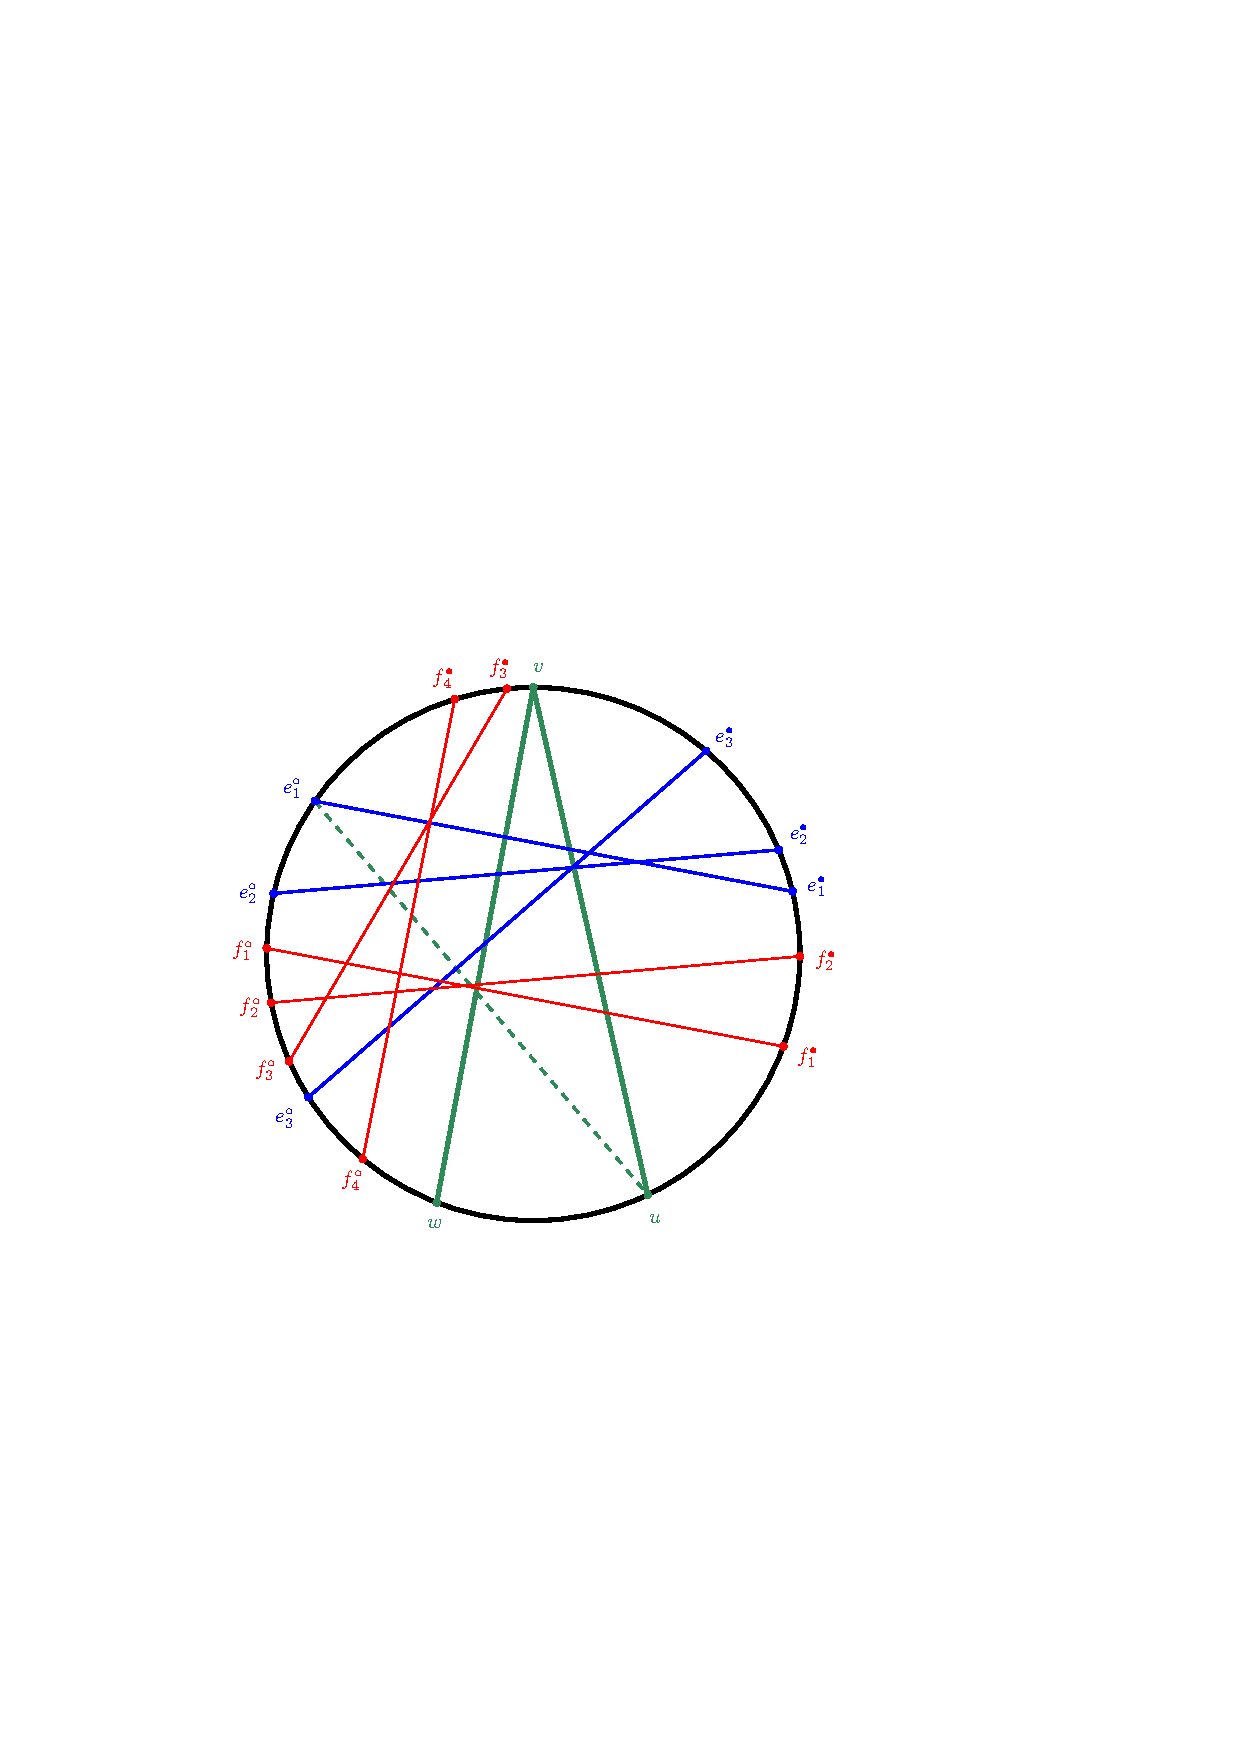
\includegraphics[width=\textwidth,page=1]{exProofStar}
  \end{subfigure}
  \begin{subfigure}[b]{.48\textwidth}
    \centering
    \includegraphics[width=\textwidth,page=2]{exProofStar}
  \end{subfigure}
  \caption{Illustrations of the first and second steps of the proof of \cref{prop:angleBelongStar}. In both case, $k=4$, and on the left, $\ell=2$.}
  \label{fig:exProofStar}
\end{figure}

\medskip
\paragraph{\bf First step.}
Suppose that $(u, e^\circ_1)$ is not in $T$. 
Since $T$ is a $k$-triangulation, there is a $k$-crossing $F=\{f_1, \dots, f_k\}$ (with $u \cl f^\bullet_1 \cl \cdots \cl f_k \cl e'_1 \cl f'_1 \cl \cdots \cl f'_k \cl u$) that prevents the diagonal~$(u, e^\circ_1)$. We will now exhibit a $(k-1)$-crossing of the form~$\{f_1, \dots, f_\ell, e_{\ell+1}, \dots, e_{k-1}\}$ that will cross~$\angle(u,v,w)$ and be $v$-farther than~$E$, contradicting the maximality of~$E$.

Note first that~$f^\bullet_k \in [v, e^\circ_1[$, as otherwise~$F \cup \{(u, v)\}$ would form a $(k + 1)$-crossing.
Additionnaly, $f^\circ_k \in {]e^\circ_1, w]}$, as otherwise $E \cup \{(v,w), (f^\bullet_k, f^\circ_k)\}$ would form a $(k + 1)$-crossing. 
Consequently, we have~$f^\circ_1 \in {]e^\circ_1, w[}$ $e^\circ_1 \cl f^\circ_1 \cl \cdots \cl f^\circ_{k-1} \cl w$.

Let $\ell = \max \set{j\in[k-1]}{\, f^\circ_i \in {]e^\circ_i, w[} \text{ for all } i \le j}$.
Then $f^\bullet_i \in {]u, e^\bullet_i]}$ for any $i \le \ell$, as otherwise $\{e_1, \dots , e_i, f_i, \dots , f_k\}$ would form a $(k + 1)$-crossing.
Thus~$f_i$ crosses~$\angle(u,v,w)$ and is $v$-farther than~$e_i$ for any~$i \le \ell$.
Furthermore, we have $f^\circ_\ell \cl f^\circ_{\ell+1} \cl e^\circ_{\ell+1}$ (by maximality of~$\ell$) and~$f^\bullet_\ell \cl e^\bullet_{\ell} \cl e^\bullet_{\ell+1}$, so that~$f_\ell$ crosses~
$e_{\ell+1}$. 
Consequently, we get a $(k-1)$-crossing $\{f_1, \dots , f_\ell, e_{\ell+1}, \dots , e_{k-1}\}$ which is $v$-farther than $\{e_1, \dots , e_{k-1}\}$, contradicting the maximality of~$E$. 
We conclude that~$(u, e^\circ_1)$ belongs to~$T$.

Suppose now that~$\angle(e^\bullet_1, e^\circ_1, u)$ is not an angle of~$T$. 
Then there exists $e^\bullet_0 \in {]u, e^\bullet_1[}$ such that $(e^\bullet_0, e^\circ_1) \in T$. 
But then the $(k-1)$-crossing $\{(e^\bullet_0, e^\circ_1), e_2, \dots, e_{k-1}\}$ is $v$-farther than~$E$. 
This implies that~$\angle(e^\bullet_1, e^\circ_1, u)$ is an angle of~$T$.

\medskip
\paragraph{\bf Second step.}
Assume now that there exists a $(k-1)$-crossing~$F=\{f_2, \dots , f_k\}$ that crosses $\angle(e^\bullet_1, e^\circ_1, u)$ and is $e^\circ_1$-farther than the $(k-1)$-crossing $\{e_2, \dots, e_{k-1}, (v, w)\}$.

Note first that~$f_k = (v,w)$. Indeed, since~$f_k$ is $e^\circ_1$-farther than~$(v,w)$, we have~$f^\bullet_k \in {]e^\bullet_1, v]}$ and~$f^\circ_k \in [w,u[$. Therefore~$f^\bullet_k = v$ (as otherwise~$\{(u,v), e_1\} \cup F$ would form a $(k+1)$-crossing), and~$f^\circ_k = w$ (since~$\angle(u,v,w)$ is an angle of~$T$).

Since~$f_k = (v,w)$, we obtain that~$\{e_1, f_2, \dots, f_{k-1}\}$ is a $(k-1)$-crossing that crosses~$\angle(u,v,w)$. For any $i \in [2,k-1]$, the diagonal~$f_i$ is $e^\circ_1$-farther than~$e_i$, and thus also $v$-farther than~$e_i$. Therefore, $\{e_1, f_2, \dots, f_{k-1}\}$ is $v$-farther than~$E$, contradicting the maximality of~$E$.
\end{proof}

Combining \cref{coro:farthestTidy} and \cref{prop:angleBelongStar}, we obtain the proof of \cref{thm:structureInfinite}\,(1):

\begin{corollary}
In a \ef \ktg of a tidy polygon, any angle belongs to a $k$-star.
\end{corollary}


\subsection{Any $k$-relevant diagonal belongs to $2$ $k$-stars, and can be flipped}

\begin{lemma}
When $k\geq 2$, any \ef \ktg of a \nbd is \vf.
\end{lemma}
\begin{proof}
Any diagonal of the $k$-border surrounding a given vertex intersects all diagonals adjacent to this vertex.
\end{proof}

\begin{lemma}
Any diagonal of a \vf \ktg belongs to $4$ angles.
\end{lemma}
\begin{proof}
The vertices adjacent to the diagonal have finite degree. Take the neighbours just before and after the other vertex. The $4$ hereby obtained diagonals form angles with the first one.
\end{proof}

\begin{lemma}
Any diagonal adjacent to $2$ $k$-star can be flipped.
\end{lemma}
\begin{proof}
cf Pilaud Santos. to be adapted to the infinite case, but shouldn't need any additional hypothesis. quite long though : section 3.
\end{proof}

\subsection{Flattening a boundary $k$-star, inflating a boundary $k$-crossing}

\begin{figure}
  \centering
  \begin{subfigure}[b]{.48\textwidth}
	\centering
	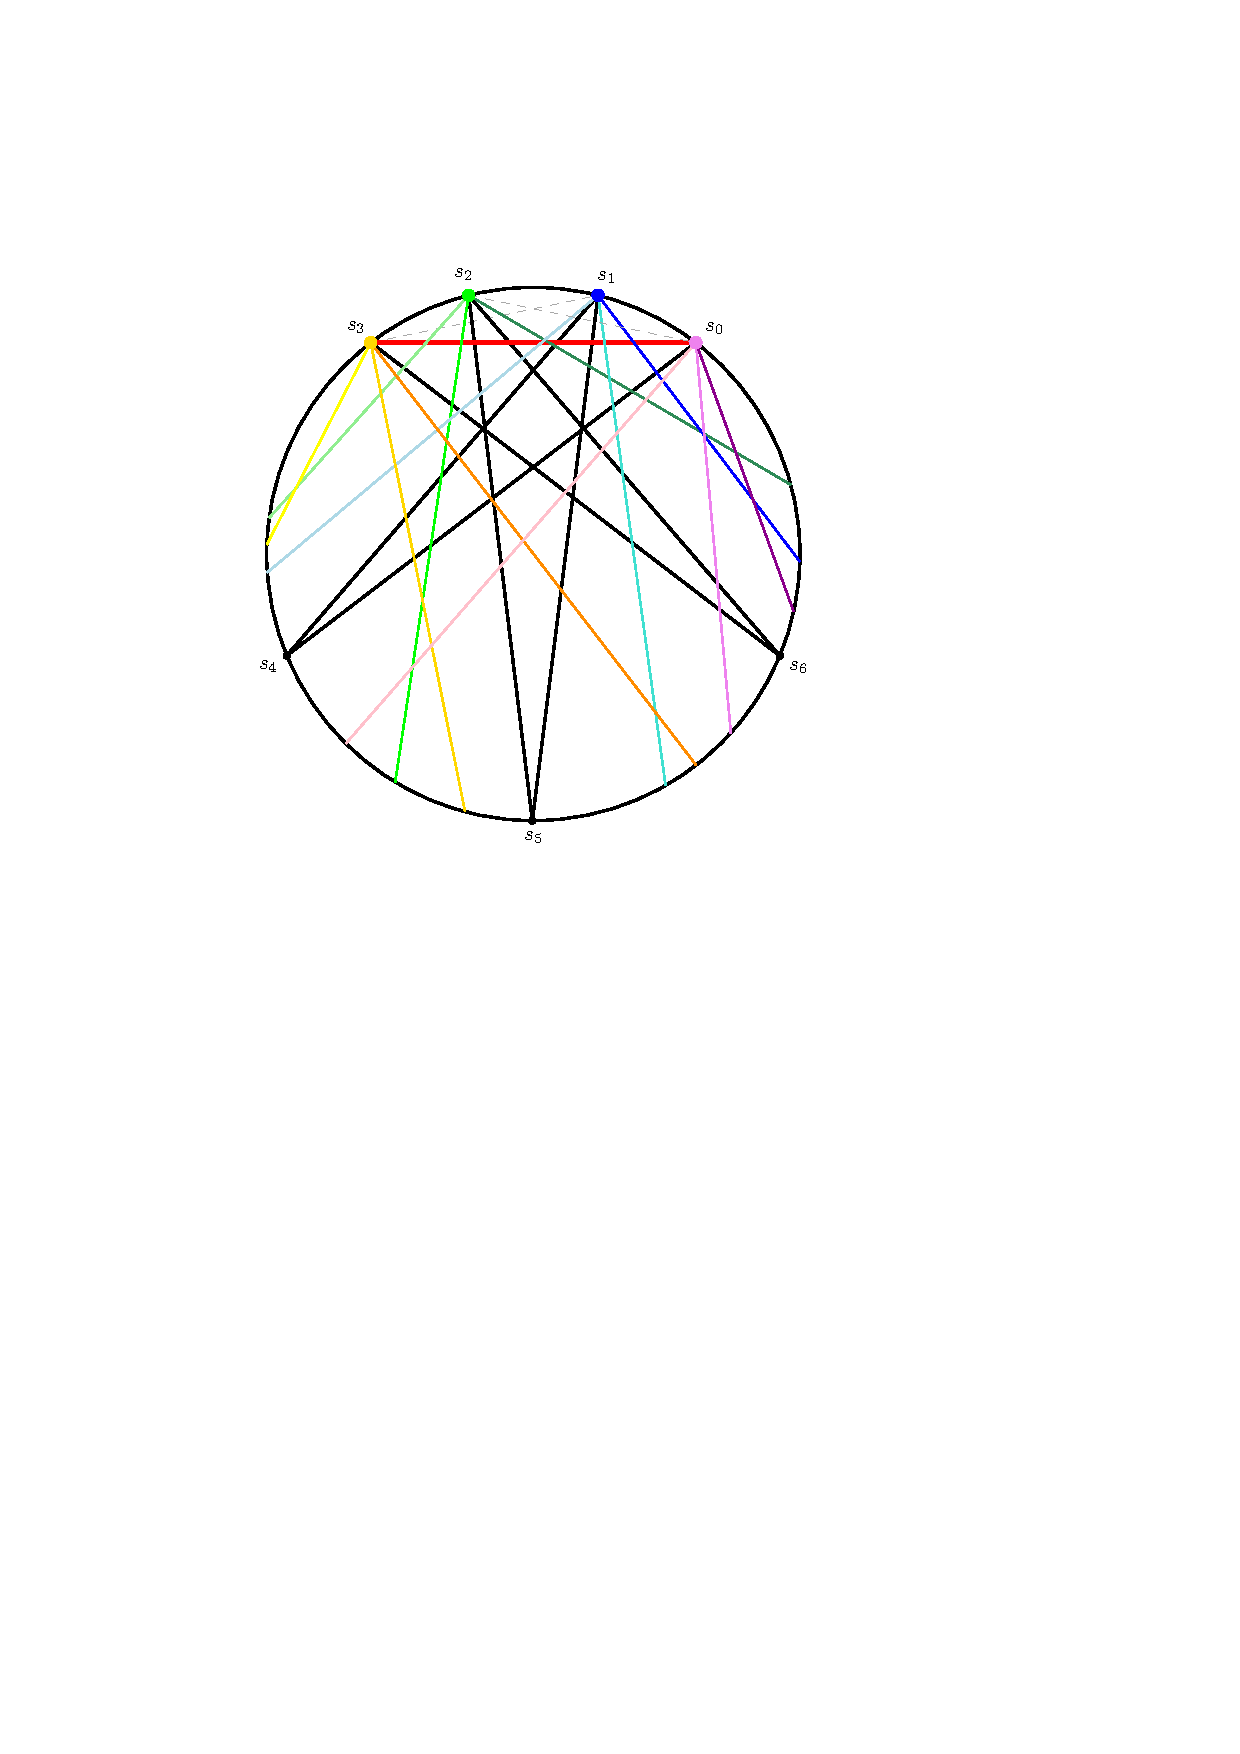
\includegraphics[width=\textwidth,page=1]{exFlattening}
  \end{subfigure}
  \begin{subfigure}[b]{.48\textwidth}
    \centering
    \includegraphics[width=\textwidth,page=2]{exFlattening}
  \end{subfigure}
  \caption{Illustrations of the flattening of a boundary $k$-star, with $k=3$.}
  \label{fig:exProofStar}
\end{figure}


\section{Some counter-examples}

\begin{ce}
The polygon of a periodic \ktg is not necessarily a \nbd.
\end{ce}
\begin{proof}

\end{proof}

\begin{ce}
A periodic \ef \ktg may have angles that are not crossed by a $(k-1)$-crossing.
\end{ce}
\begin{proof}

\end{proof}

\begin{ce} 
A periodic \ktg may not be \ef.
\end{ce}
\begin{proof}

\end{proof}

\begin{ce}
A \ef \ktg of a \nbd is not necessarily \vf.
\end{ce}
\begin{proof}
k=1
\end{proof}



\bibliographystyle{abbrv}
\bibliography{../bibliography}

\end{document}
